% !TEX TS-program = pdflatex
% !TEX encoding = UTF-8 Unicode

% This is a simple template for a LaTeX document using the "article" class.
% See "book", "report", "letter" for other types of document.

\documentclass[11pt]{article} % use larger type; default would be 10pt

\usepackage[utf8]{inputenc} % set input encoding (not needed with XeLaTeX)
\usepackage[english]{babel}

\usepackage[style=numeric, backend=bibtex]{biblatex}
\addbibresource{bibliography.bib}

%%% Examples of Article customizations
% These packages are optional, depending whether you want the features they provide.
% See the LaTeX Companion or other references for full information.

%%% PAGE DIMENSIONS
\usepackage{geometry} % to change the page dimensions
\geometry{a4paper} % or letterpaper (US) or a5paper or....
% \geometry{margin=2in} % for example, change the margins to 2 inches all round
% \geometry{landscape} % set up the page for landscape
%   read geometry.pdf for detailed page layout information

\usepackage{graphicx} % support the \includegraphics command and options
\usepackage{float}
\graphicspath{ {images/} }
\usepackage{wrapfig}
\usepackage{rotating}
\usepackage{tikz}
% \usepackage[parfill]{parskip} % Activate to begin paragraphs with an empty line rather than an indent

%%% PACKAGES
\usepackage{booktabs} % for much better looking tables
\usepackage{array} % for better arrays (eg matrices) in maths
\usepackage{paralist} % very flexible & customisable lists (eg. enumerate/itemize, etc.)
\usepackage{verbatim} % adds environment for commenting out blocks of text & for better verbatim
\usepackage{subfig} % make it possible to include more than one captioned figure/table in a single float
% These packages are all incorporated in the memoir class to one degree or another...

%%% HEADERS & FOOTERS
\usepackage{fancyhdr} % This should be set AFTER setting up the page geometry
\pagestyle{fancy} % options: empty , plain , fancy
\renewcommand{\headrulewidth}{0pt} % customise the layout...
\lhead{}\chead{}\rhead{}
\lfoot{}\cfoot{\thepage}\rfoot{}

%%% SECTION TITLE APPEARANCE
\usepackage{sectsty}
\allsectionsfont{\sffamily\mdseries\upshape} % (See the fntguide.pdf for font help)
% (This matches ConTeXt defaults)

%%% ToC (table of contents) APPEARANCE
\usepackage[nottoc,notlof,notlot]{tocbibind} % Put the bibliography in the ToC
\usepackage[titles,subfigure]{tocloft} % Alter the style of the Table of Contents
\renewcommand{\cftsecfont}{\rmfamily\mdseries\upshape}
\renewcommand{\cftsecpagefont}{\rmfamily\mdseries\upshape} % No bold!

%%% EXTRA Packages
\usepackage{listings}
\renewcommand{\lstlistingname}{Code}% Listing -> Code
\renewcommand{\lstlistlistingname}{List of \lstlistingname s}
\usepackage{xcolor}

%For Figuers and labels
\usepackage[english]{babel}


\lstset{
    string=[s]{"}{"},
    stringstyle=\color{blue},
    comment=[l]{:},
    commentstyle=\color{black},
	breaklines=true,
	postbreak=\mbox{\textcolor{red}{$\hookrightarrow$}\space}
}

%%% END Article customizations

%%% The "real" document content comes below...

\title{Modernizing Legacy Software (Concluder Web Application)}
\author{Hashem Alsaggaf}
%\date{} % Activate to display a given date or no date (if empty),
         % otherwise the current date is printed 

\begin{document}
\maketitle
\tableofcontents


\section{Introduction}
The purpose of this paper is to document the process of developing the first version of a web application.\\[24pt]
Subjects mentioned or discussed and attachments in this paper:
\begin{itemize}
\item Pairwise Comparison Method
\item Normalization
\item Matrix calculations
\item Tree structure
\item html codes
\item javascript codes
\item jQuery codes
\item JSON Objects
\item Design sketches
\item Developing method
\item Implementation highlights
\item Logic Diagram
\item Screenshots
\item Current Issues
\item Room for enhancement
\end{itemize}

\subsection{Project Background}
In 2016, a team of developers and researchers contributed to create \textit{Concluder}. An open source java software, developed to calculate inconsistency in order to improve decision making and knowledge management by employing Pairwise Comparison method for weight distribution. Screenshots of the software can be seen in Figure \ref{shot:oldConcluder}.



\begin{sidewaysfigure}
    \centering
   
      	 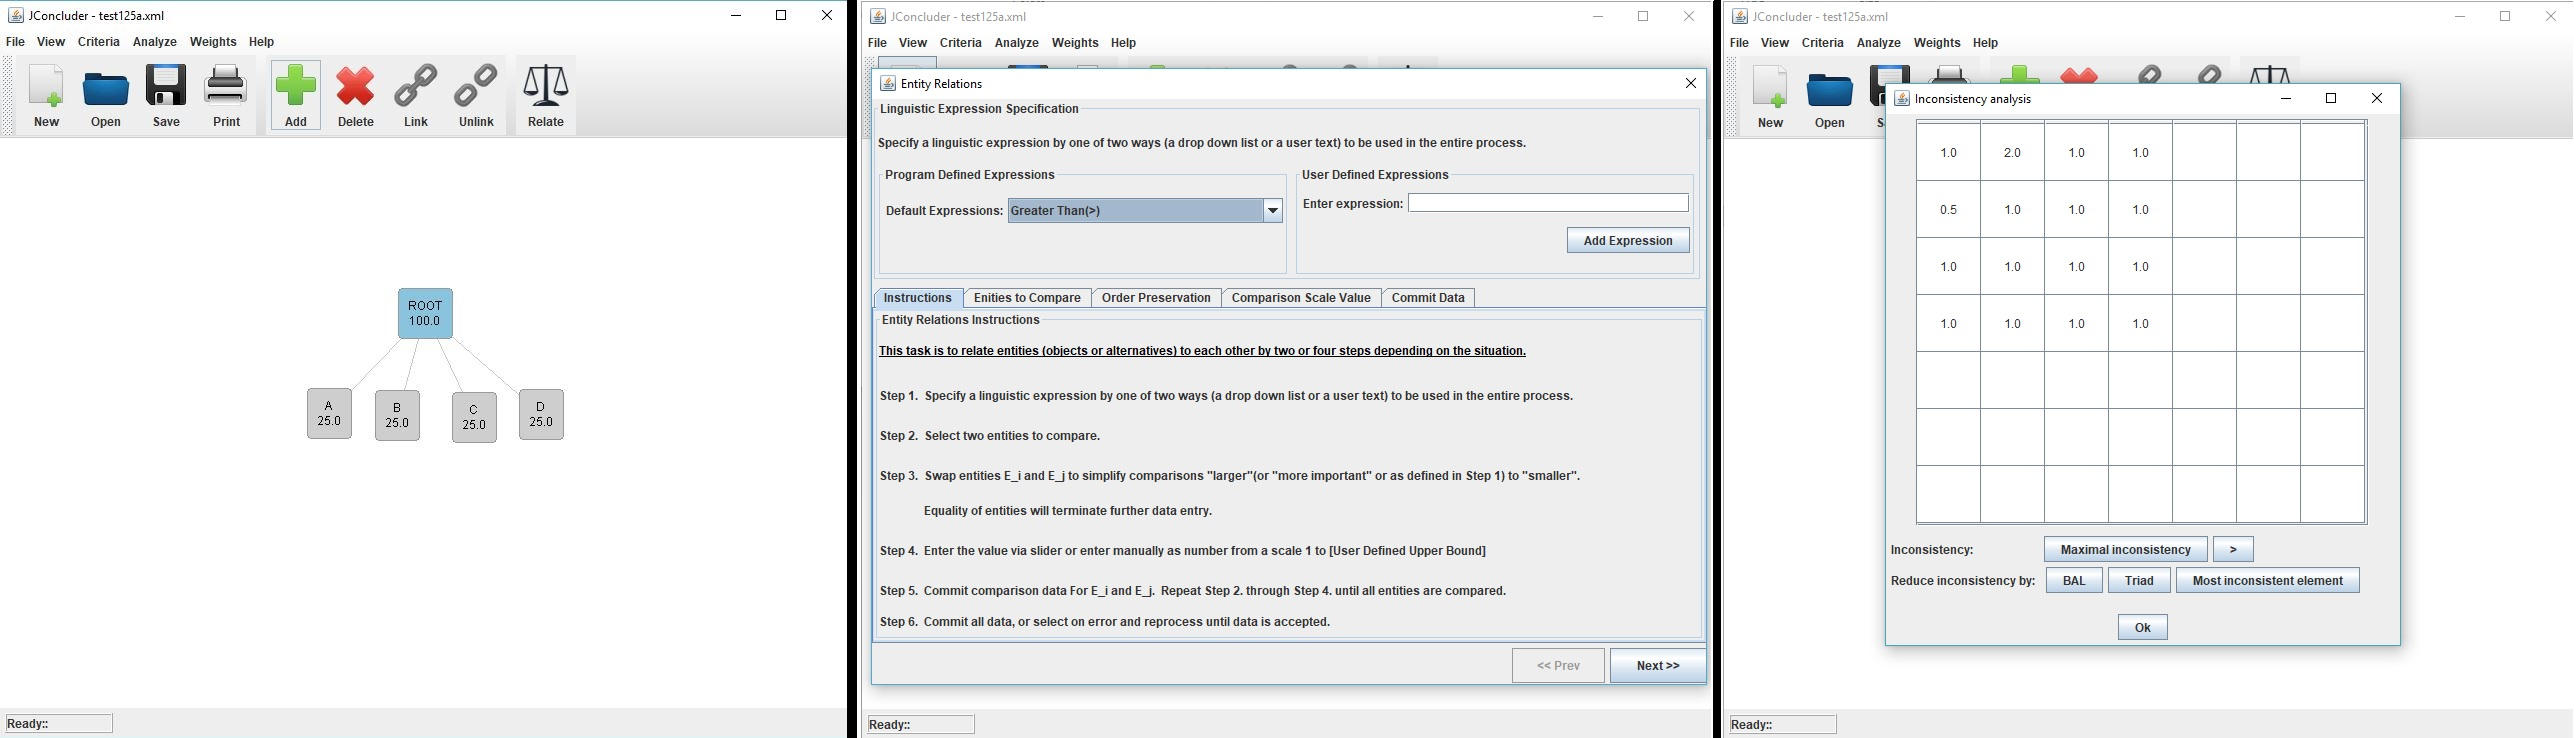
\includegraphics[width=\linewidth]{concluder}
    
    \caption{Screenshots of the java version of Concluder}
    \label{shot:oldConcluder}
\end{sidewaysfigure}

\subsection{Goal}
The goal of this project is to design and implement a web application version of Concluder. This version should be accessible from any device with modern internet browser.

\section{Developing Method}

The developing method of this project consists of five phases:
\begin{itemize}
\item System requirements
\item UI/UX design
\item Implementation
\item testing
\item publishing
\end{itemize}

\section{System requirements}
In this phase, a list of Concluder web application features will be identified. To understand the system requirements, we looked at the java version of Concluder, then highlighted most of its features, keeping in mind that more features will be added as the development cycle iterate.
Some of the features are:
\begin{itemize}
\item Elements representation
\item Editing elements
\item Elements relations
\item Calculating and reducing Inconsistency
\end{itemize}


\subsection{Elements representation}
One of the most important requirement is a way to represent elements. In the java version of Concluder, elements are represented as a tree (see Figure \ref{shot:oldConcluder}).  The user would likely expect to see elements represented as a tree in the web application as well. Therefore, elements should be represented as a tree in the web app version of Concluder.

\subsection{Editing elements}
Another required feature is to be able to manipulate the elements. That includes adding new elements to the tree, editing existing nodes in the tree, and deleting nodes from the tree.

\subsection{Elements relations}
Another main feature is to be able to relate elements by weights. Elements relation need to be represented as weights in this version as well.

\subsection{Calculating and reducing Inconsistency}
The Pairwise Comparison Method calculates inconsistency using matrices. The minimum required calculations are:

\begin{itemize}
\item Presenting Pairwise Comparison (PC) matrix.
\item Weight distribution.
\item Relation inconsistency.
\item Reducing inconsistency.
\item Normalization.
\end{itemize}

\section{UI/UX Design}
In this phase, a number of sketches for the  user interface and experience is produced to guide the implementation phase. After that, the user interface will be designed with Webflow.io to produce clean HTML and CSS files to be used as a wire-frame for the application.

\subsection{webflow.io}
Webflow.io is a cloud-based software as a service (SaaS). It is used to visually make responsive web page designs.\\
The use of such a tool is necessary to be able to design and edit the user interface rapidly and in a fast way. One main advantage of using webflow.io is the ability to export the design to HTML/CSS/JS code. The exported code is simple, organized, and very easy to read and understand. Once the code is exported, it is treated as a wire-frame for the UI.

\subsection{Design details}
To accommodate an organized user interface, the design of different windows (called screens) is proposed. The main screens are Edit Screen, Relation Screen, and Analyzing Screen. As seen in Figure \ref{sketch:basic screen} and in figure \ref{sketch:realtionScreenSketch}, in each screen, there is different control buttons and/or panels. To navigate between screens, a slide panel on the left side of the application is designed (called Main Panel), look at Figure \ref{screenshot:tree editing}.

\begin{sidewaysfigure}
   	\centering
    	\caption{Edit Tree Sketch}
 	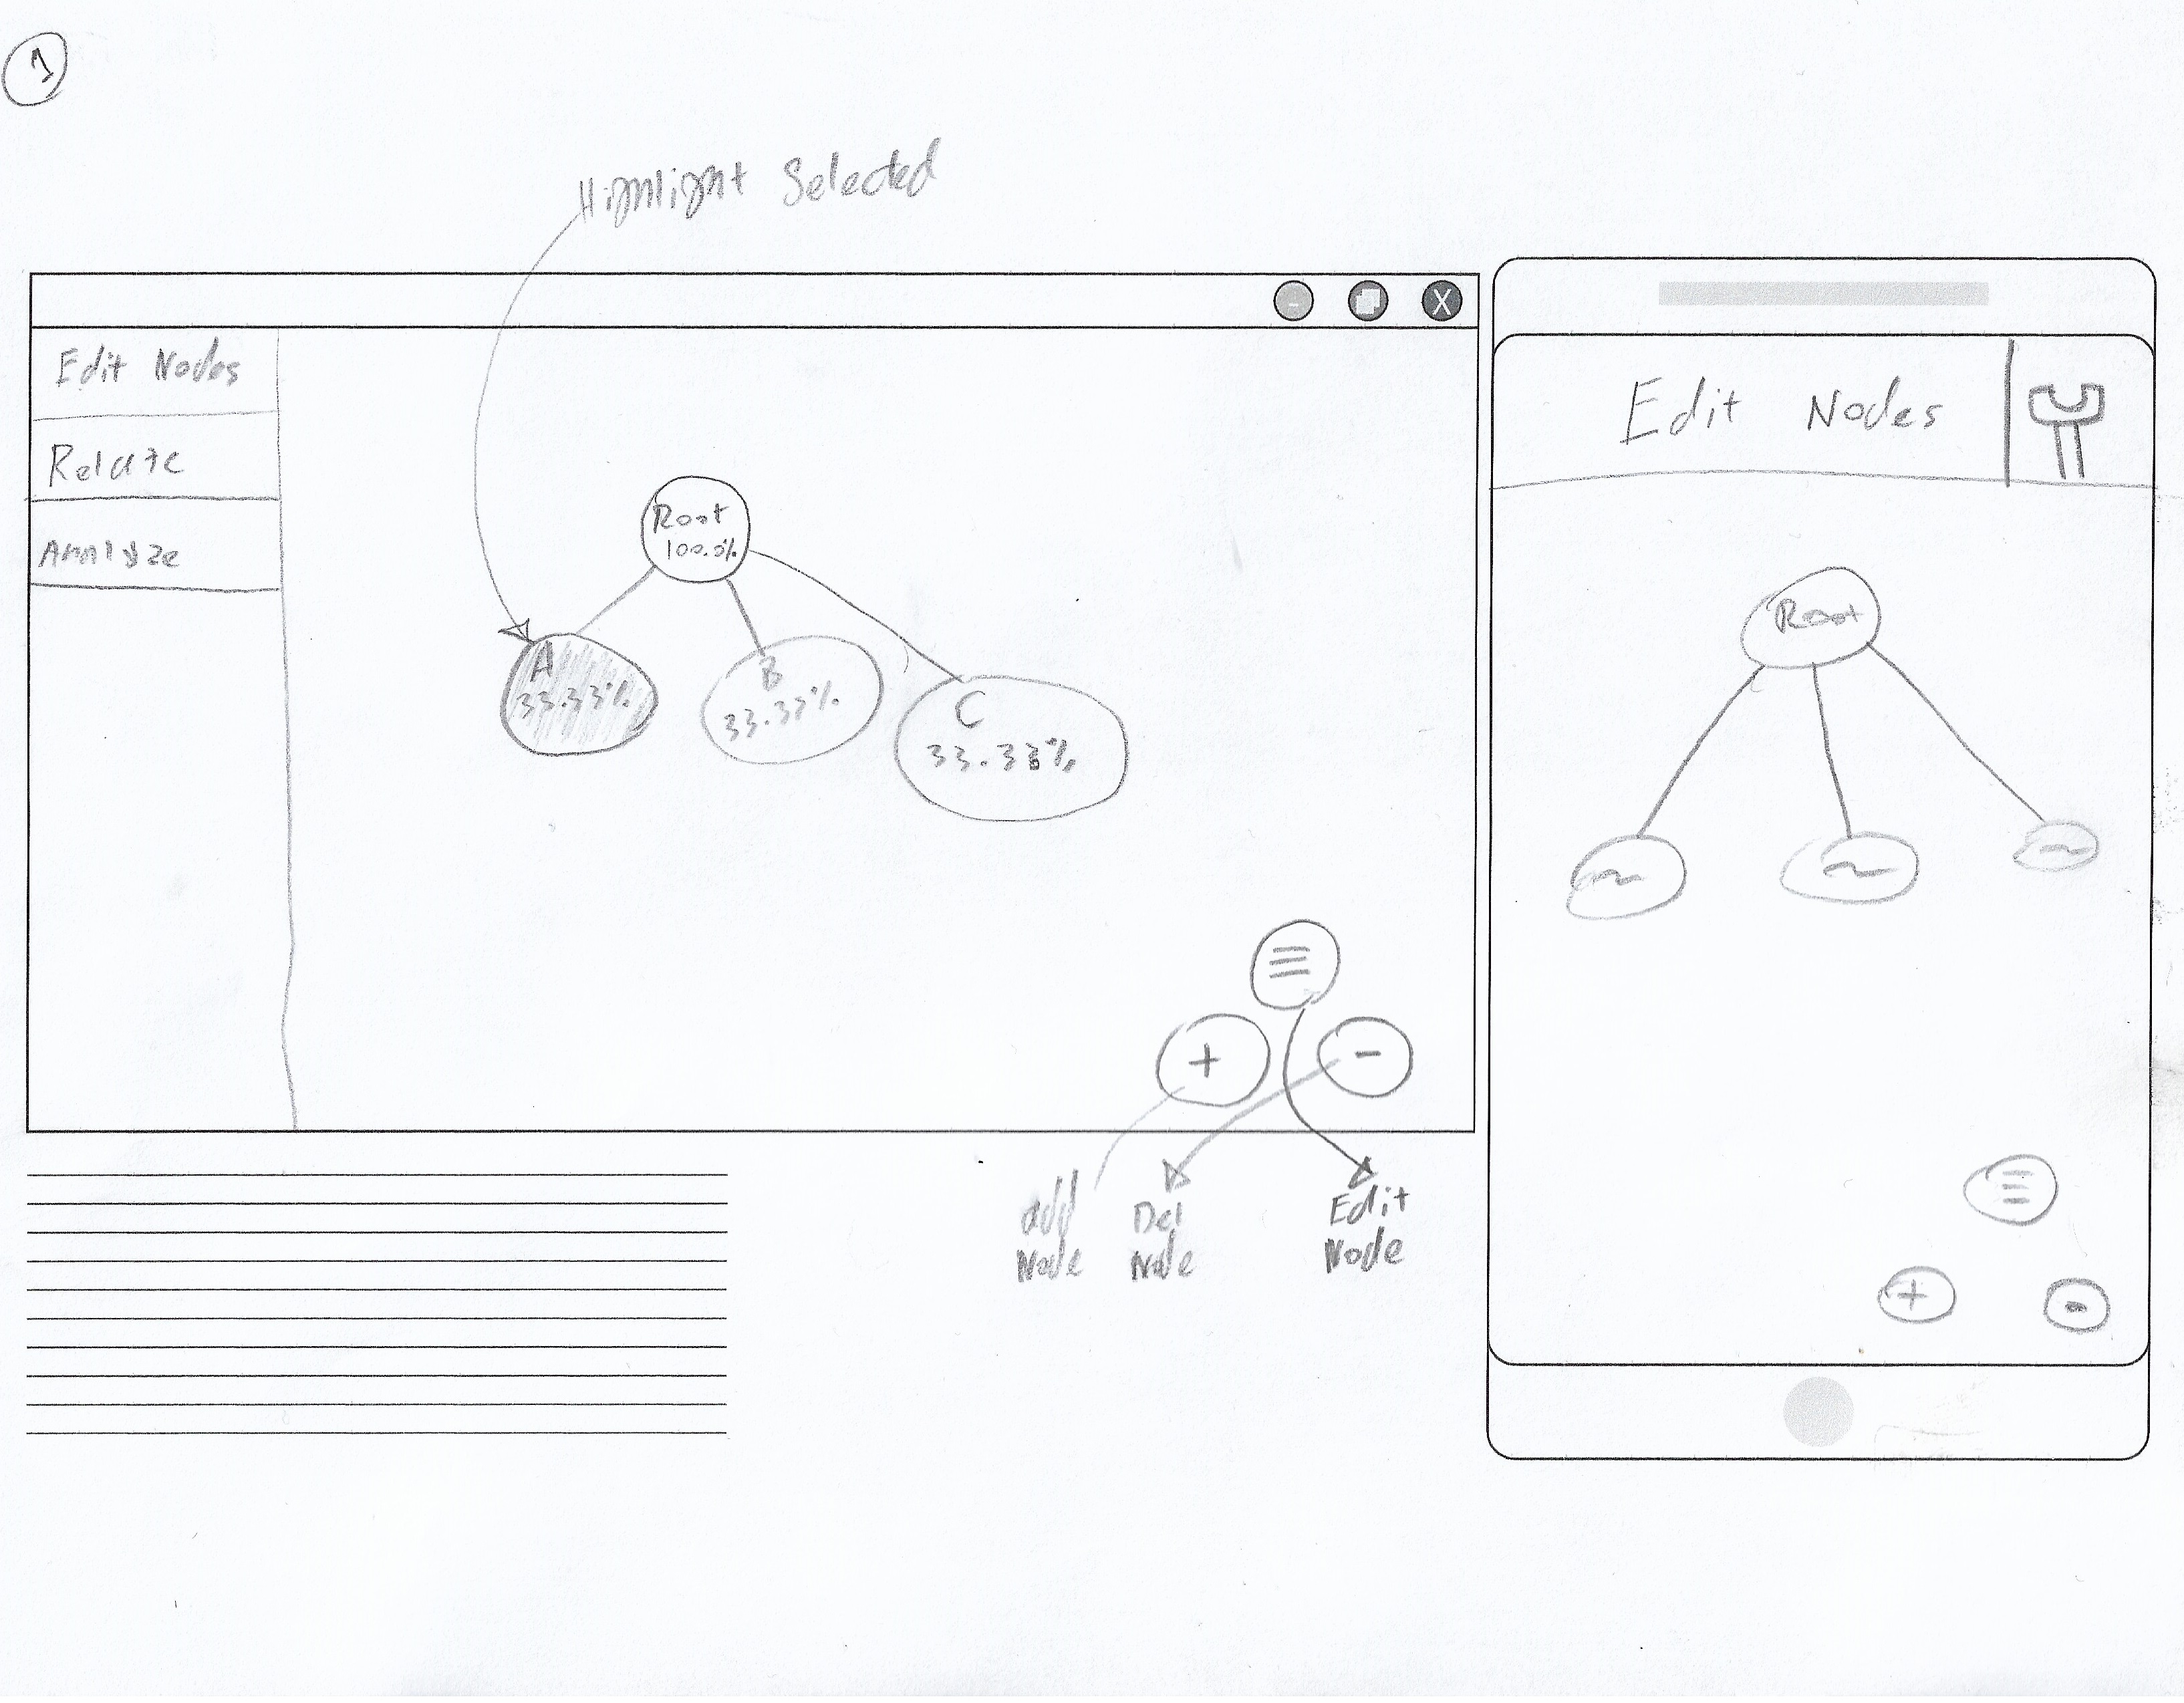
\includegraphics[width=\linewidth]{skitchScreens}
    
    \label{sketch:basic screen}
\end{sidewaysfigure}



\begin{sidewaysfigure}
  \caption{Tree Editing screenshot}
  \centering
  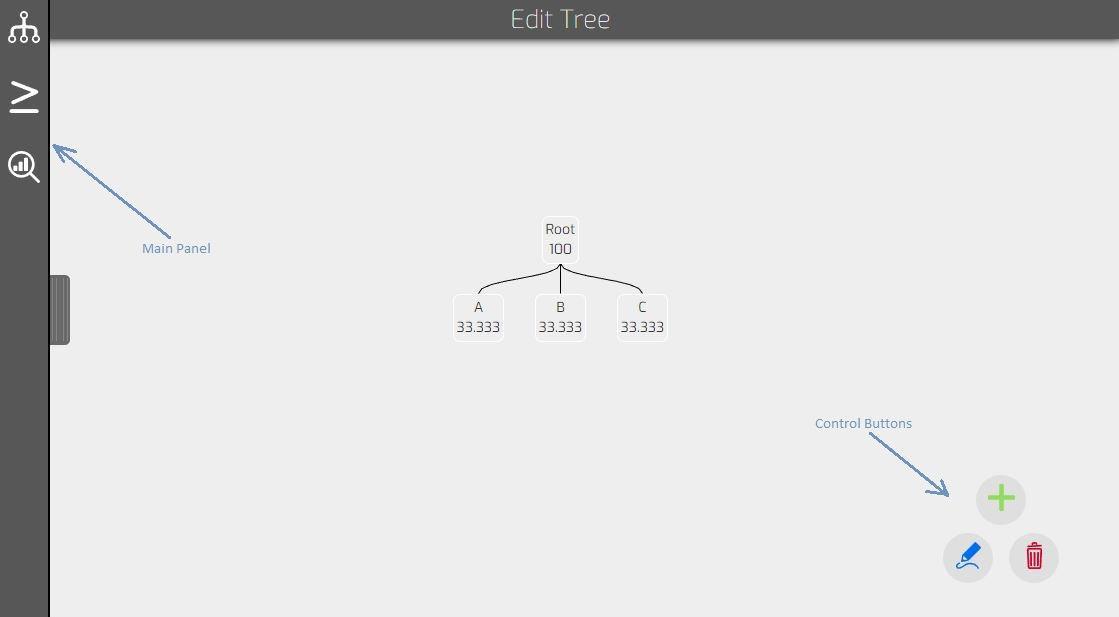
\includegraphics[width=\linewidth]{editTreeScreenshot}
  \label{screenshot:tree editing}
\end{sidewaysfigure}

\noindent For user feedback, a pop-up window, with a theme that matches the overall theme is designed, see Figure \ref{screenshot:message}. This window will provide help and tips to the user when needed.

\begin{figure}[h!]
  \caption{Messaging Example}
  \centering
  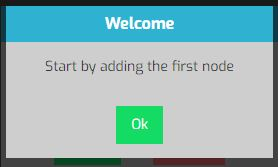
\includegraphics[width=0.7\textwidth]{message}
  \label{screenshot:message}
\end{figure}

\subsubsection{Edit Screen}
This is where the user interact with the tree structure in terms of adding, editing, or deleting nodes from the tree.
As the system requires the manipulating of a tree structured data, we need to design a layout where the user can view the tree and manipulate it at the same time. At the bottom right of this screen, the user can see three buttons with declarative icons; add, delete and edit. See Figure \ref{screenshot:tree editing}. Before any action is committed, the user confirmation is needed to avoid accidental actions. See Figure \ref{diagram:editScreenAction} for an example of the user flow in terms of editing the tree.

\begin{figure}
  \caption{Add a node flow diagram}
  \centering
  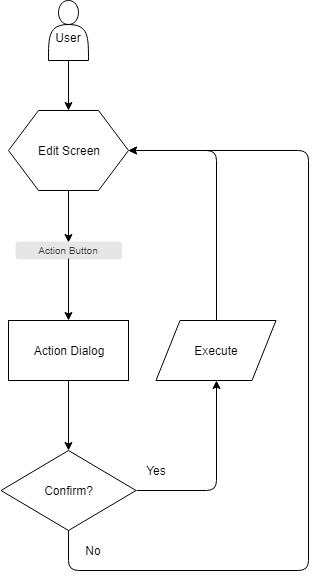
\includegraphics[width=0.7\textwidth]{editScreenAction}
  \label{diagram:editScreenAction}
\end{figure}

\noindent
The same flow principle applies on deleting and editing nodes.

\subsubsection{Relation Screen}\label{relation screen}
A sketch for this screen is presented in Figure \ref{sketch:realtionScreenSketch}. In this screen, the user is able to see the tree and select two nodes to set the relation between them, see Figure \ref{screenshot:relation screen}. When two nodes are selected, the Relation Wizard will show the two selected nodes, and will ask the user to choose which node is bigger and by how much, see Figure \ref{screenshot:relation wizard}. After applying the relation between two nodes, the relation will be saved in the Nodes Relations tab. To access the Nodes Relations tab, the user would click on the Relations Tab Button at the bottom right-corner of the screen, see Figure \ref{screenshot:relation screen}.
In the Nodes Relations tab, the user have the ability to Edit or Delete a relation, see Figure \ref{screenshot:relation tab}. See the diagram in Figure \ref{diagram:relationFlow} for the user flow in Relation Screen.

\begin{sidewaysfigure}
   	\centering
    	\caption{Relations Sketch}
 	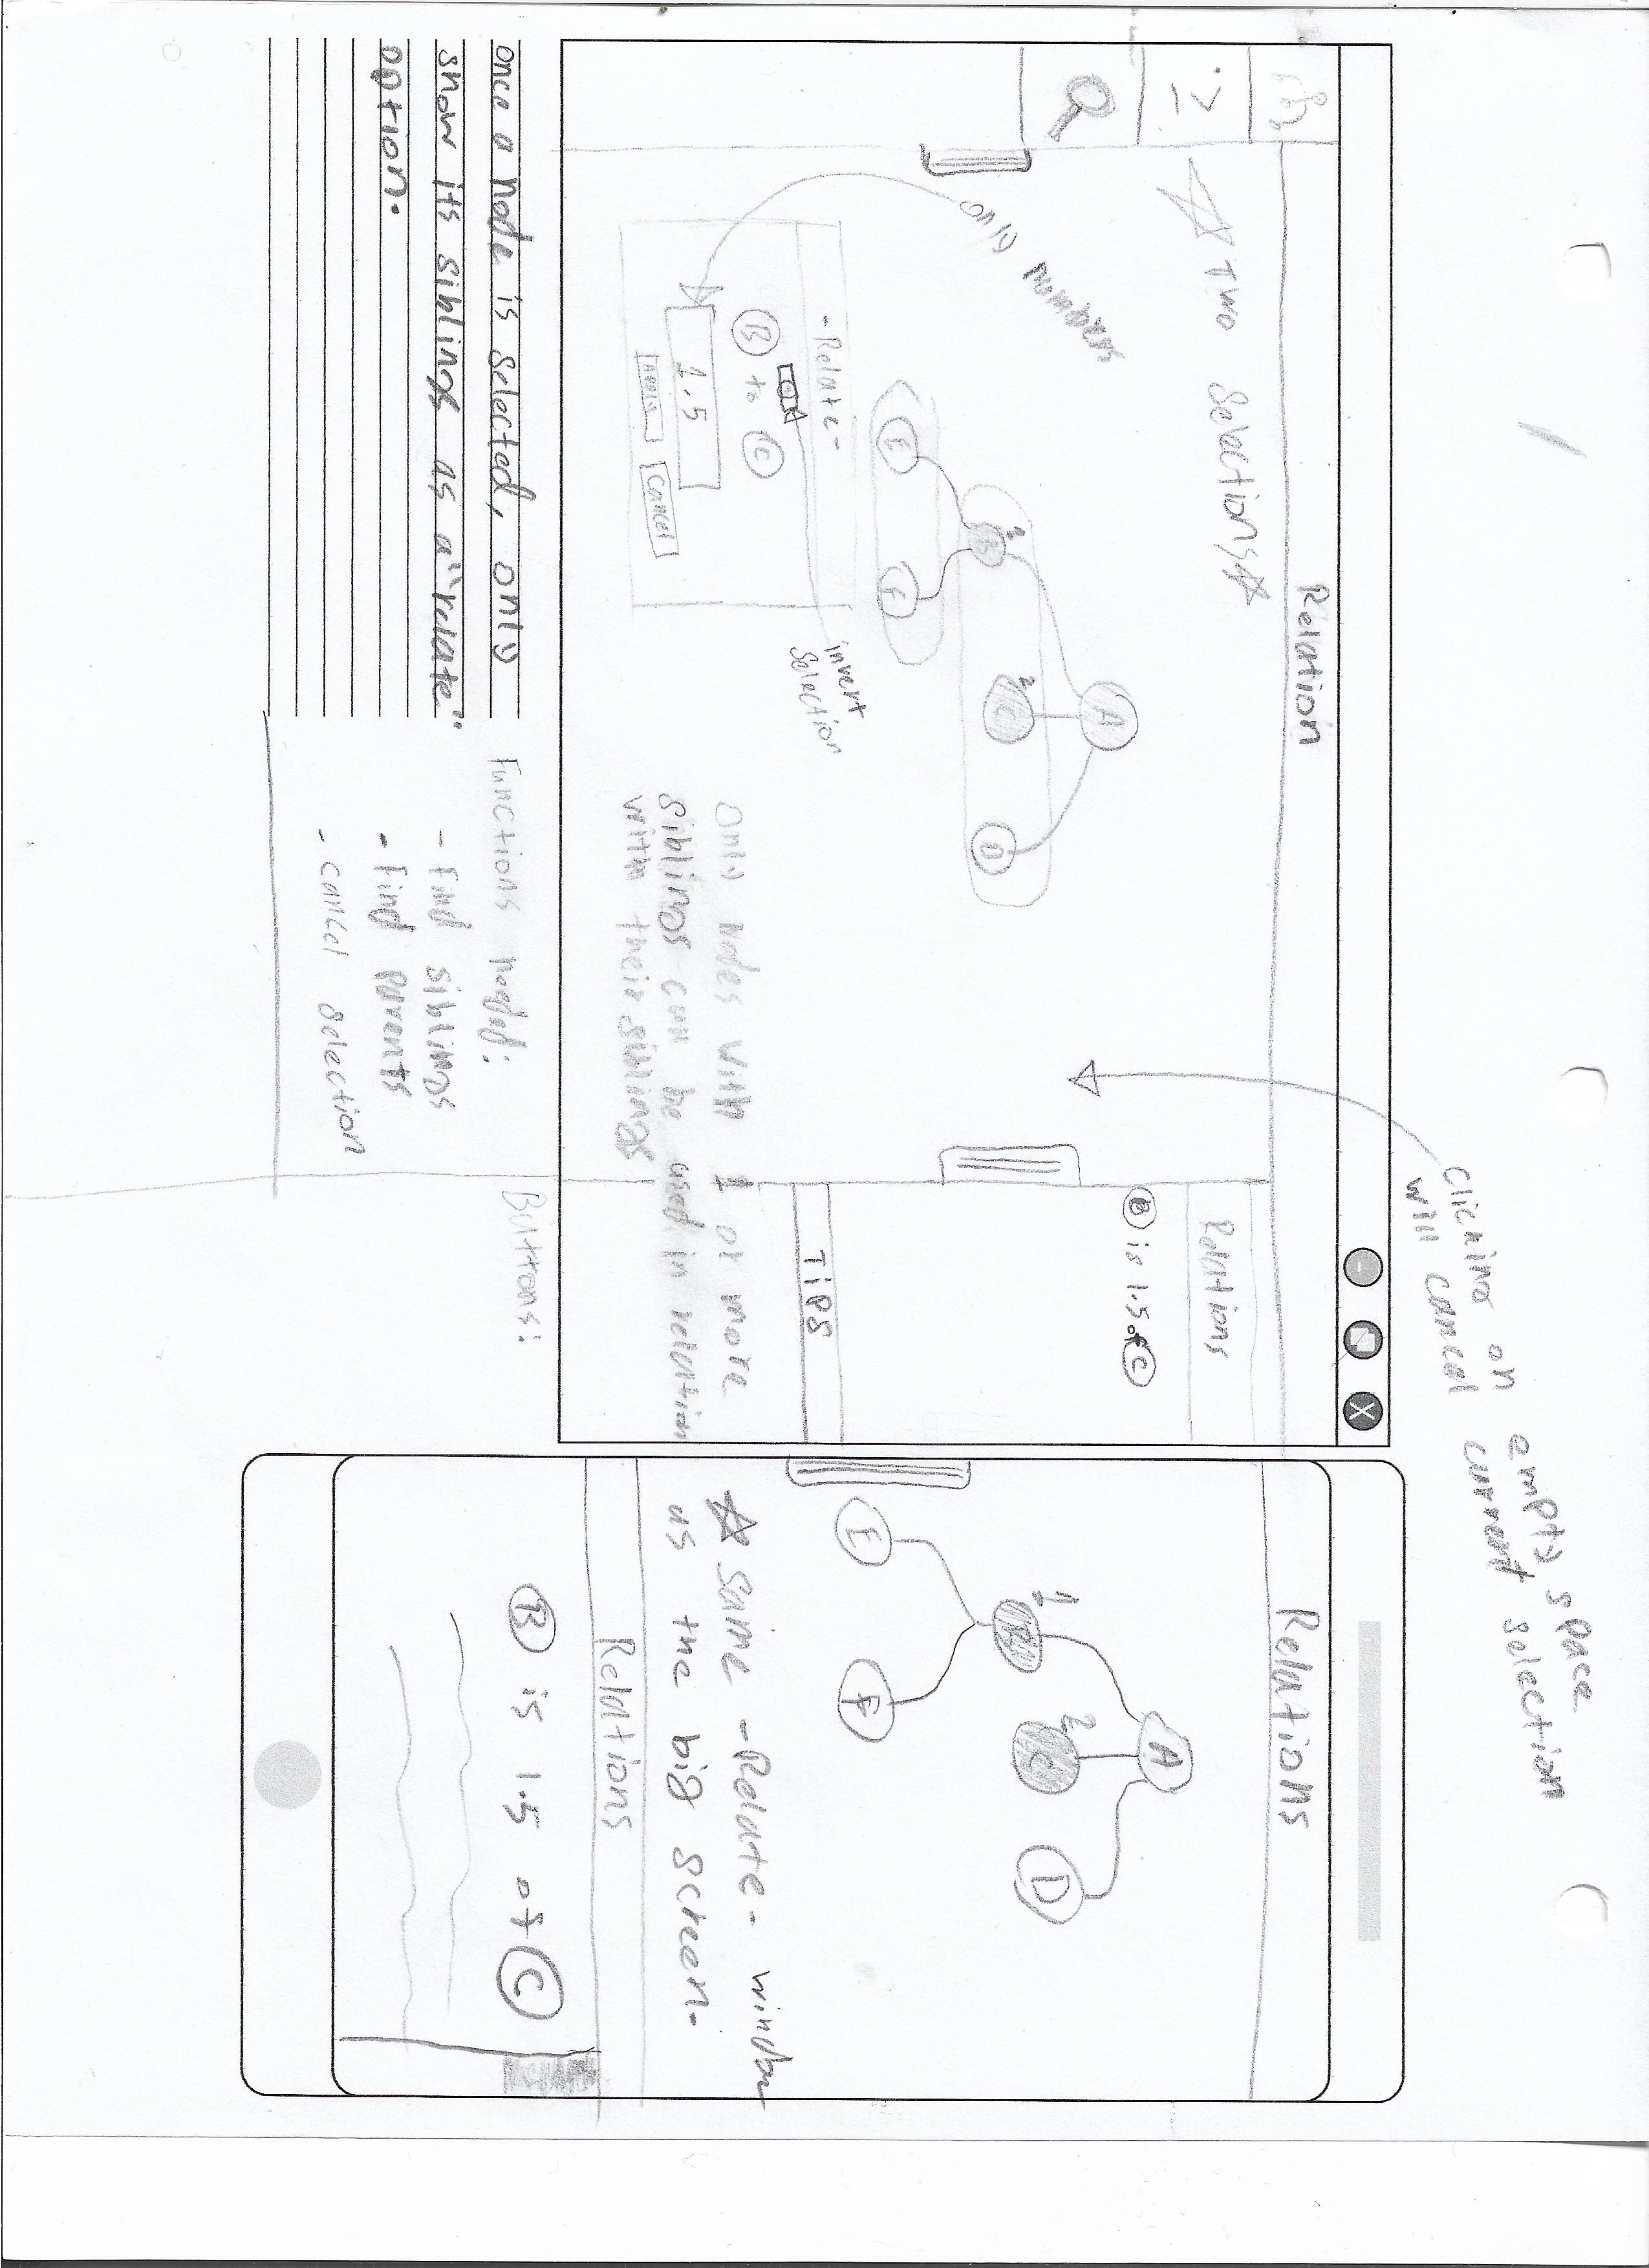
\includegraphics[width=0.75\linewidth, angle=90]{realtionScreenSketch}
    
    \label{sketch:realtionScreenSketch}
\end{sidewaysfigure}

\begin{sidewaysfigure}
  \caption{Relation Screen screenshot}
  \centering
  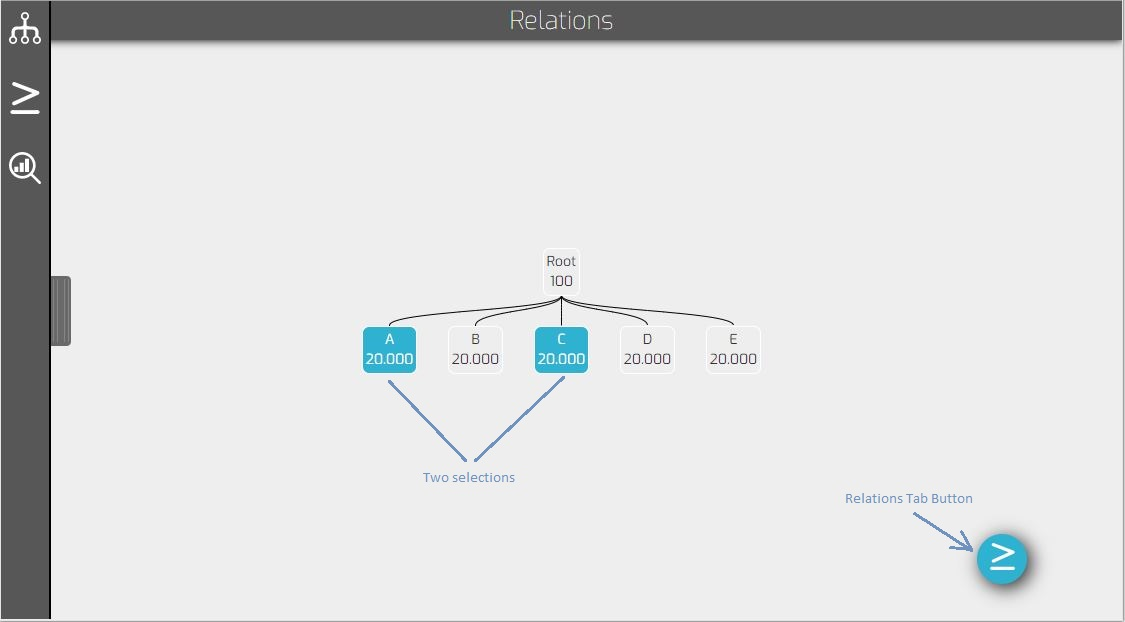
\includegraphics[width=\textwidth]{relationScreenshot}
  \label{screenshot:relation screen}
\end{sidewaysfigure}

\begin{sidewaysfigure}
  \caption{Relation Wizard}
  \centering
  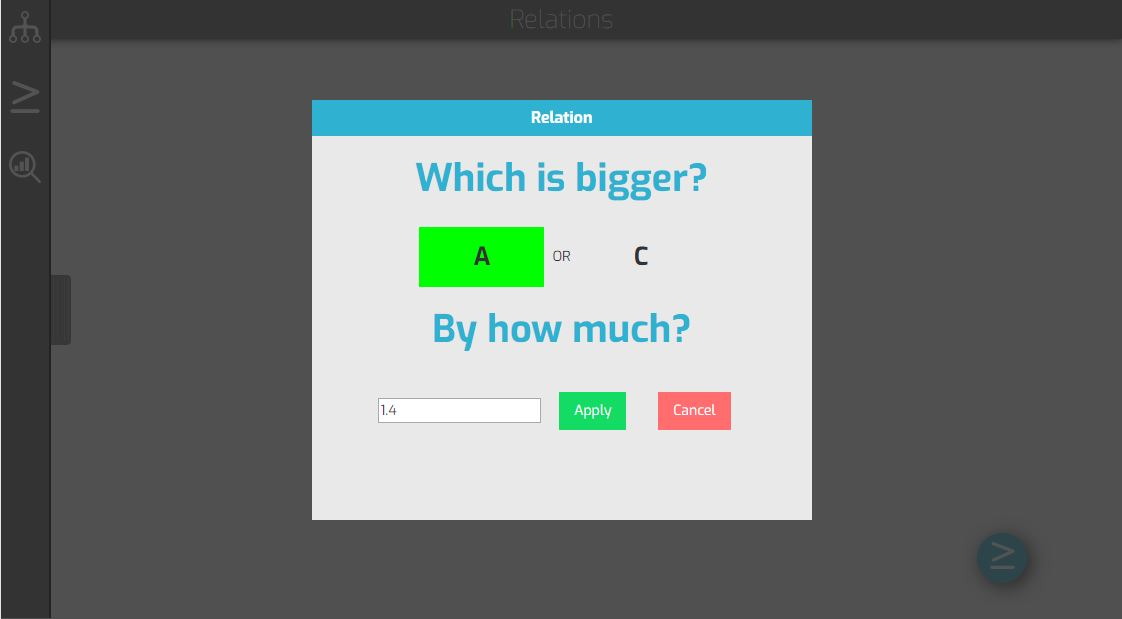
\includegraphics[width=\textwidth]{relationWizard}
  \label{screenshot:relation wizard}
\end{sidewaysfigure}

\begin{sidewaysfigure}
  \caption{Relation Tab}
  \centering
  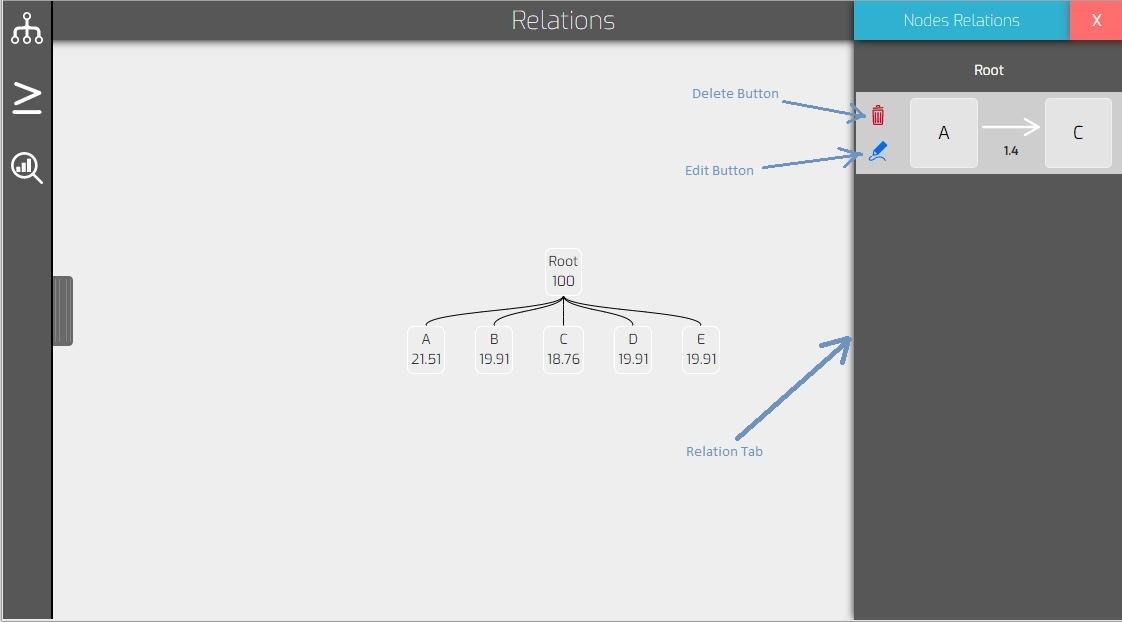
\includegraphics[width=\textwidth]{relationTab}
  \label{screenshot:relation tab}
\end{sidewaysfigure}

\begin{figure}
  \caption{Relation (User Flow)}
  \centering
  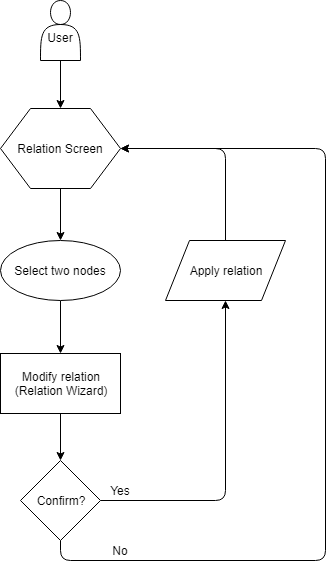
\includegraphics[width=0.7\textwidth]{relationFlow}
  \label{diagram:relationFlow}
\end{figure}

\newpage
\subsubsection{Analyzing Screen}
When the user navigate to this screen, the user will see the tree where all nodes with three or more children are highlighted, see Figure \ref{screenshot:analyze Highlight}. When the user click on a highlighted node, the Analyze Wizard will show and present an editable relation matrix (Editable Pairwise Comparison Matrix) for that group, see Figure \ref{screenshot:analyze wizard}.\\[24pt]



\begin{figure}[h!]
  \caption{Nodes with children}
  \centering
  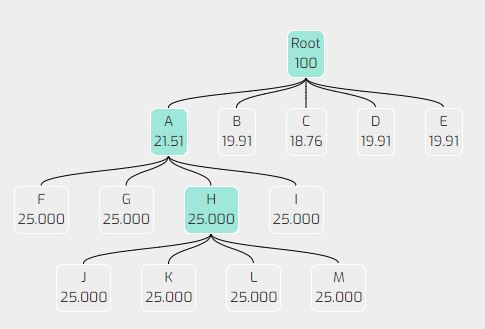
\includegraphics[width=\textwidth]{analyzeScreenHighlights}
  \label{screenshot:analyze Highlight}
\end{figure}

\begin{sidewaysfigure}
  \caption{Analyze Wizard}
  \centering
  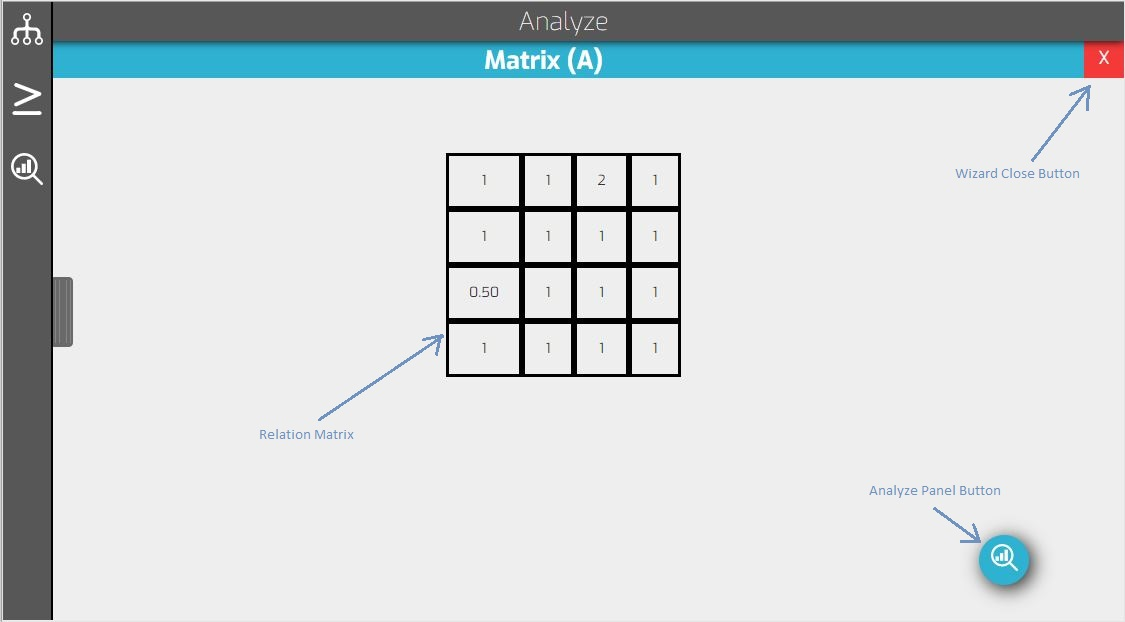
\includegraphics[width=\textwidth]{analyzeWizard}
  \label{screenshot:analyze wizard}
\end{sidewaysfigure}
\noindent
In the Analyze Wizard, the user is able to analyze the matrix by using the Analyze Panel. The Analyze Panel is accessible by clicking on the Analyze Panel button at the bottom-right corner of the Analyze Wizard, see Figure \ref{screenshot:analyze wizard}.\\
See diagram in Figure \ref{diagram:analyzeUserFlow} to get an overview of the user flow in the Analyze Screen.

\begin{figure}
  \caption{Analyze Screen User Flow}
  \centering
  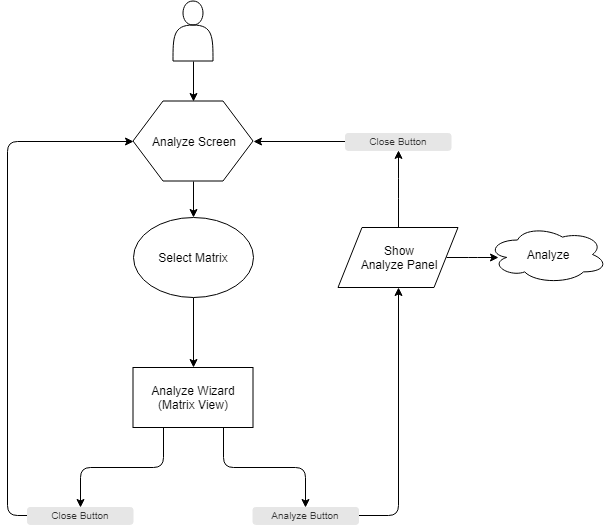
\includegraphics[width=\textwidth]{analyzeUserFlow}
  \label{diagram:analyzeUserFlow}
\end{figure}

\noindent
The analyze panel has two sections; General and Traids. See Figure \ref{screenshot:analyze panel}.

\begin{sidewaysfigure}
  \caption{Analyze Panel}
  \centering
  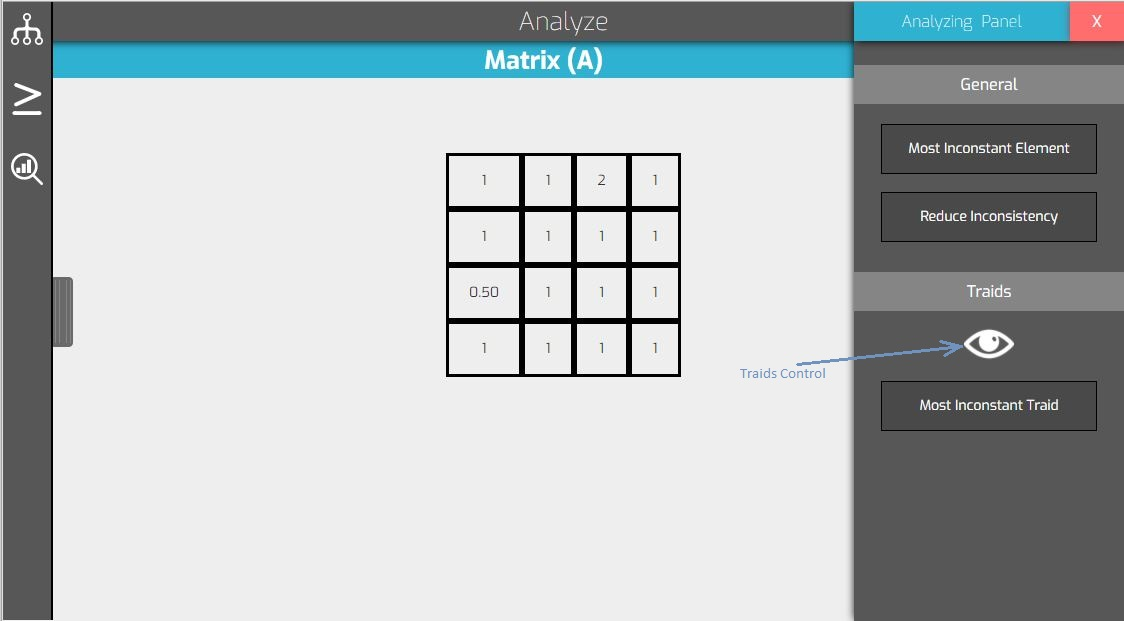
\includegraphics[width=\textwidth]{analyzePanel}
  \label{screenshot:analyze panel}
\end{sidewaysfigure}

\begin{itemize}
\item General section has general analyzing functions, like showing the most inconsistent elements and reducing inconsistency button.
\item Traid section deals with traids analyzing operations, like showing all traids, reducing a traid, and showing the most inconsistent traid.
\end{itemize}

\noindent
When clicking on the Traid Control button, the first traid will be highlighted in the matrix, the traids counter and total number of traids will be presented, the inconsistency value will also be presented, and the traid navigation button and the Hide traid button will show as well. See Figure \ref{screenshot:analyze traid control}.

\begin{sidewaysfigure}
  \caption{Analyze Panel - Traid Control}
  \centering
  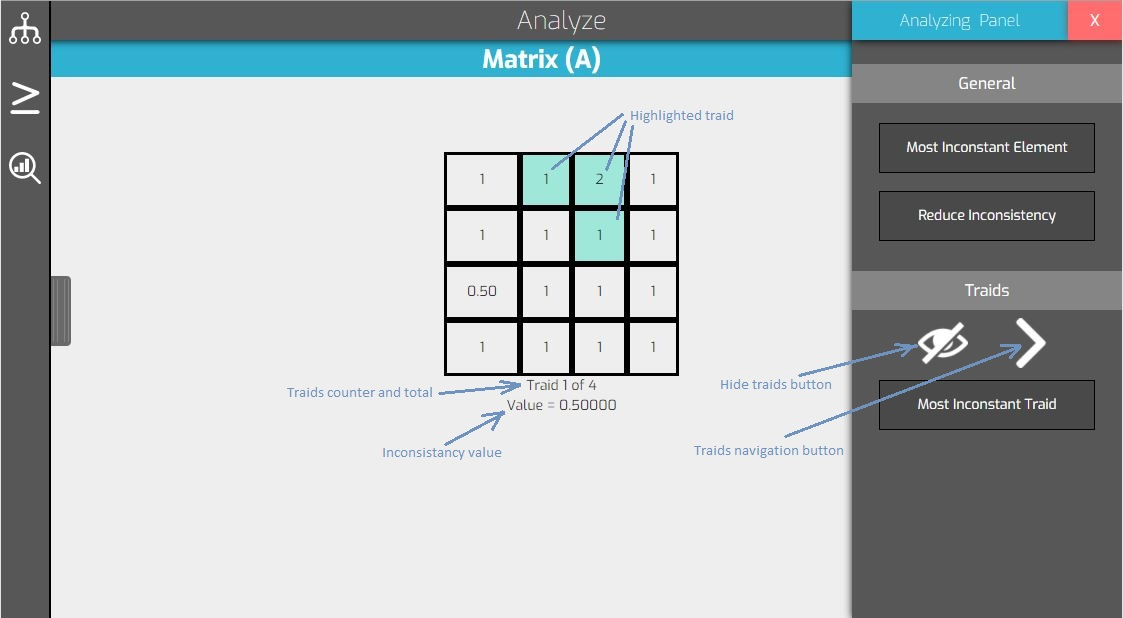
\includegraphics[width=\textwidth]{analyzeTraidControl}
  \label{screenshot:analyze traid control}
\end{sidewaysfigure}

\newpage
\section{Implementation}
In this phase, The UI is taken from sketches and designed in webflow.io. after the UI is designed, a clean html and css code is produced and used as a wire-frame for the project.\\
After producing the html and css codes, some html elements are given an ID to be accessible by javascript. The ID assignments is critical to be able to do things like showing different screens and wizards, assign actions to buttons, etc...\\
For this project, all screens are hidden by default (the css display property is set to `none'). To show a screen, the screen and the button related to that screen is given an html id. Then an action to show the screen is programmed to be triggered when the button is clicked.
Lets consider the Relation Screen for example. Take a look at the html code for the Relation Screen and its button, See Code \ref{code:relationBtnHtml}.

\noindent
\begin{minipage}[c]{\linewidth}
\begin{lstlisting}[basicstyle=\scriptsize, tabsize=4, frame=single, caption= Relation Button html code, label=code:relationBtnHtml]

<div id="relationIcon" class="menu-btn">
	<img src="images/relation.svg" class="menu-icon" />
</div>
...
...
...
<div id="relationScreen" class="relations-screen">
	...
	...
	...
</div>
\end{lstlisting}
\end{minipage}
\noindent
Notice \textbf{id=''relationIcon''} and \textbf{id=''relationScreen''}. Also, take a look at the javascript (js) code (Code \ref{code:relationIconClick})\footnote{jQuery library is used here.} to see how we are showing the Relation Screen when the Relation icon/button is clicked.\\
\noindent
\begin{minipage}[c]{\linewidth}
\begin{lstlisting}[basicstyle=\scriptsize, tabsize=4, frame=single, caption= Relation Button html code, label=code:relationIconClick]

var relationIcon = $('#relationIcon');
var relationScreen = $('#relationScreen');

relationIcon.click(function(){
	relationScreen.show();
}
                    
\end{lstlisting}
\end{minipage}
\noindent
This technique is implemented for most buttons in this project.\\[12pt] \noindent
Sometimes we have to hide and show screens based on events too. For example, we have to hide the Analyzing Screen when the user navigates away from it.\\[6pt]

\begin{minipage}[c]{\linewidth}
To ensure easier readability of coeds and easier maintenance, the code for each feature is placed in a separate file. We have the following files:

\begin{itemize}
\item nodes.js - deals with trees and nodes operations
\item matrix.js - deals with matrix operations
\item relation.js - deals with relation's operation
\item analyze.js - deals with analyzing tasks
\item control.js - deals with UI buttons and control
\item index.js - deals with screen navigation, shortcuts, etc...
\end{itemize}
\end{minipage}
\\[12pt]

\noindent The js files are listed in `index.html' as a script resources, in a sequence where the bottom js files have access to all variables and function in the js files above it. However, those are not the only js files in the application, we are also using jQuery and Treant.js libraries.

\subsection{Elements Representation (tree structure)}
Elements representation is one of the most important aspect of this system. Elements are represented as a tree structure, we used Treant.js\footnote{  Treant.js is a javascript library that create tree structure charts from JSON objects.}. With Treant.js, we need an HTML div with ID (where the tree will be represented) and a JSON object (the tree we want to represent). The JSON object should have the following structure.

\begin{minipage}[c]{\linewidth}
\begin{lstlisting}[basicstyle=\scriptsize, tabsize=4, frame=single, caption= Tree Example, label=code:tree example]
Tree = {
    chart: {
        container: "#tree-simple"
    },
    
    nodeStructure: {
        text: { name: "Parent node" },
        children: [
            {
                text: { name: "First child" }
            },
            {
                text: { name: "Second child" }
            }
        ]
    }
};
\end{lstlisting}
\end{minipage}
\noindent The above JSON tree structure (Code \ref{code:tree example}) will produce the following chart (Figure \ref{simple tree output}).

\begin{figure}[h!]
  \caption{Simple tree output}
  \centering
  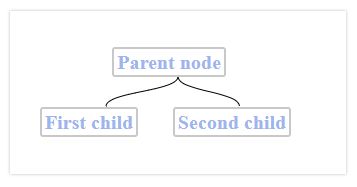
\includegraphics{simpleTreeExample}
  \label{simple tree output}
\end{figure}

\noindent Note: each node in the tree chart is an HTML div element, this is important for tree manipulation.

\subsubsection{Tree Configuration}\label{tree configuration}
The two main attribute for a tree object (as described in treant-js library website) are:
\begin{itemize}
\item chart (JSON pair values)
\item nodeStructure (JSON pair values)
\end{itemize}

\noindent
In \textbf{chart} attribute, we set the chart configuration. For the purpose of this software, we made use of the following attributes for chart configuration:

\begin{itemize}
\item container
\item node
\item callback
\end{itemize}

\noindent To access the container attribute, we use \textbf{Tree.chart.container}. In the \textbf{container} attribute, we declare the html div ID where the tree will be drawn.
Example: To change the div where the tree is drawn (Code \ref{code:tree container}):

\begin{lstlisting}[basicstyle=\scriptsize, tabsize=4, frame=single, caption= Tree container example, label=code:tree container]
Tree.chart.container = "#treeDiv";
\end{lstlisting}

\noindent In the above example (Code \ref{code:tree container}), the tree will be drawn in an html div with the ID `treeDiv' (notice the number sign before the ID)
\\[12pt]
\noindent In the \textbf{node} attribute, we made use of the key `HTMLclass'.

\begin{itemize}
\item HTMLclass is used to apply a CSS class to every node in the tree (remember, all nodes are html elements)
\end{itemize}

\noindent Example:
\begin{lstlisting}[basicstyle=\scriptsize, tabsize=4, frame=single, caption=Tree.node Example, label=code:tree.node example]
node: {
	HTMLclass: "nodeClick",
},
\end{lstlisting}

\noindent In the above example (Code \ref{code:tree.node example}), a class called `nodeClick` is applied to every node.

\noindent In \textbf{callback} attribute, we can set javascript functions and events. All events are listed in the Treant-js websites. We made use of the event `onTreeLoaded` to apply a function that is triggered when a node is clicked (Code \ref{code:nodeClick function}).
\\[12pt]
\noindent
\begin{minipage}[c]{\linewidth}
\begin{lstlisting}[basicstyle=\scriptsize, tabsize=4, frame=single, caption=Node click trigger function, label=code:nodeClick function]
callback: {
	onTreeLoaded :  function(){
		$('.nodeClick').click(function(){
			...
		});
	}
},
\end{lstlisting}
\end{minipage}


\noindent A complete chart configuration would look like this (Code \ref{code:completeChartConfig})

\noindent
\begin{minipage}[c]{\linewidth}
\begin{lstlisting}[basicstyle=\scriptsize, tabsize=4, frame=single, caption= Chart configuration, label=code:completeChartConfig]
treeConfig = {
	chart: {
		container: "#treeDiv",
		node: {
			HTMLclass: "nodeClick",
		},
		callback: {
			onTreeLoaded : function(){
				$('.nodeClick').click(function(){
					...
					...
					...
				});
			}
		}
	}
}
\end{lstlisting}
\end{minipage}

A complete code for tree configuration is shown in Code \ref{code:completeTreeConfig}.

\noindent
\begin{minipage}[c]{\linewidth}
\begin{lstlisting}[basicstyle=\scriptsize, tabsize=4, frame=single, caption= Complete Tree Configuration, label=code:completeTreeConfig]
var treeConfig = {
	    chart: {
        container: "",
		node: {
			HTMLclass: "nodeClick"
		},
		callback: {
			onTreeLoaded : function(){
				$('.nodeClick').click(function(){
					clearSelection();
					$(this).css({'background-color': '#2fb1d1', 'color': 'white'});
					selectedNode = $(this).attr('id');
					findNode(selectedNode);// for debugging
				});
			}
		}
    },
    
    nodeStructure: {
		HTMLid: "node_root",
        text: { name: "Root",  weight: 100},
		parent: "",
        children: [
			
		],
		matrix: [
		
		]
    }
};

\end{lstlisting}
\end{minipage}

\subsubsection{Tree Structure}
In the \textbf{`nodeStructure`}, we define the structure of the tree, in terms of children and descriptive text. A very simple structure could be like the one shown in (Example - Code \ref{code:tree container}).  Every node has parents excepts the root node. All children of a node are listed in the children attribute (as an array), and a descriptive text is set in the text attribute.\\
\noindent
For this project, some extra attributes has been introduced; \textbf{HTMLid, parent, and matrix}, see Code \ref{code:nodeStructure}.

\noindent
\begin{minipage}[c]{\linewidth}
\begin{lstlisting}[basicstyle=\scriptsize, tabsize=4, frame=single, caption=nodeStructure code, label=code:nodeStructure]
nodeStructure: {
	HTMLid: "node_root",
	text: { name: "Root",  weight: 100},
	parent: "",
	children: [
			
	],
	matrix: []
}
\end{lstlisting}
\end{minipage}

\subsection{Editing elements - Tree operations}
First thing we need to do is to draw the tree using treant.js library functions. The basic code to draw the tree is shown in Code \ref{code:basicTreeDraw}. To keep the tree configuration intact and to make sure we can always reset a tree configuration, we clone the tree configuration (`treeConfig') as our tree (see Code \ref{code:jqueryExtend}). Note that the variable `treeConfig' is already defined as a tree configuration with chart settings and nodes structure (See Code \ref{code:completeChartConfig}).\\[6pt]

\noindent
\textbf{'\$.extend'} is a jQuery function that is used to merge tow objects together. By merging any object with an empty object, we get a cloned object. The overhead of cloning is necessary to keep our tree settings intact, in case we need to reset the tree.

\noindent
\begin{minipage}[c]{\linewidth}
\begin{lstlisting}[basicstyle=\scriptsize, tabsize=4, frame=single, caption=\$.extend syntax, label=code:jqueryExtend]
var Tree = $.extend(true, {}, treeConfig);
\end{lstlisting}
\end{minipage}



\noindent
\begin{minipage}[c]{\linewidth}
\begin{lstlisting}[basicstyle=\scriptsize, tabsize=4, frame=single, caption=Basic Tree Drawing, label=code:basicTreeDraw]
chart = new Treant(Tree, function() { }, $);
\end{lstlisting}
\end{minipage}
\noindent
However, the tree will need to be drawn in multiple locations across the software. Therefore, a function called `\textbf{drawTree}' is implemented, see Code \ref{code:drawTree function}.

\noindent
\begin{minipage}[c]{\linewidth}
\begin{lstlisting}[basicstyle=\scriptsize, tabsize=4, frame=single, caption=drawTree Function, label=code:drawTree function]
function drawTree(target ,tree){
	tree.chart.container = target;
	chart = new Treant(tree, function() { }, $);
}
\end{lstlisting}
\end{minipage}

\noindent
\textbf{drawTree} function takes tow arguments; \textbf{target} and \textbf{tree}. \textbf{target} is the div id where the tree will be drawn, and \textbf{tree} is the tree we want to draw.\\
Now we can use this function to draw trees in different screens.\\[12pt]

\noindent
Second, we need a mechanism to select a node in the tree, meaning we need to find a way for the software to know what node the user is selecting.

\noindent
The steps for selecting a node are:
\begin{itemize}
\item A mapping table is created to store references of each node
\item When a node is created, an id will be assigned for it
\item A reference to the new node is stored in the mapping table
\item A variable called `\textbf{selectedNode}' is created to store the id of a selected node
\item The user clicks on a node
\item The software then look for that node in the mapping table by its id
\item The node id will be stored in `\textbf{selectedNode}'
\item As a feedback, the background of the selected node is changed.
\end{itemize}

\noindent
These steps involves many aspects. We already implemented the click trigger for all nodes (see Code \ref{code:nodeClick function}), now we need to define the actions for the trigger. However, we have different screens, and each screen uses the click trigger for different actions. For example, in the Edit Screen, we just select the node to specify where the new node will be listed or which node to delete, but in the Relation Screen, we can select two nodes to relate between them.
To accommodate different use for the same trigger, we can access the callback attribute and change the action. Refer to \ref{tree configuration} for tree configuration.\\

\noindent
When the Edit Screen is visible, the callback attribute holds the code shown in Code \ref{code:callbackEditScreen}.

\noindent
\begin{minipage}[c]{\linewidth}
\begin{lstlisting}[basicstyle=\scriptsize, tabsize=4, frame=single, caption=callback code for Edit Screen, label=code:callbackEditScreen]
callback: {
	onTreeLoaded : function(){
		$('.nodeClick').click(function(){
			clearSelection();
			$(this).css({'background-color': 'gray', 'color': 'white'});
			selectedNode = $(this).attr('id');
			findNode(selectedNode);
		});
	}
}


\end{lstlisting}
\end{minipage}

\noindent
The function \textbf{clearSelection()} will simply reset the background of all nodes in the tree. See Code \ref{code:clearSelection}.

\noindent
\begin{minipage}[c]{\linewidth}
\begin{lstlisting}[basicstyle=\scriptsize, tabsize=4, frame=single, caption=clearSelection Function, label=code:clearSelection]

function clearSelection(){
	$('.node').each(function(){
		$(this).css({'background-color': 'gray', 'color': 'black'}); 
	});
}

\end{lstlisting}
\end{minipage}

\noindent


\noindent
We might need to access the root of our tree in some situations. Therefore, we need to assign a root variable as shown in Code \ref{code:rootAssignment}.

\noindent
\begin{minipage}[c]{\linewidth}
\begin{lstlisting}[basicstyle=\scriptsize, tabsize=4, frame=single, caption=Root assignment, label=code:rootAssignment]
var root = Tree.nodeStructure;
\end{lstlisting}
\end{minipage}
\\[12pt]
\noindent
Editing elements now becomes a matter of accessing and manipulating the tree structure. To access any node in the tree, we can use the mapping table. The mapping table, is initialized with the root reference (see Code \ref{code:mapInit}), and every time a node is added, a refrence to that node is added in the mapping table as well.

\noindent
\begin{minipage}[c]{\linewidth}
\begin{lstlisting}[basicstyle=\scriptsize, tabsize=4, frame=single, caption=Mapping the tree root, label=code:mapInit]
var map = {
	'node_root': root
};

\end{lstlisting}
\end{minipage}

\noindent
We have three main operations for manipulating the tree;

\begin{itemize}
\item Add Node
\item Edit Node
\item Delete Node
\end{itemize}

\subsubsection{Adding nodes}
To add a new node, we first need to have an id counter to make sure all ids are unique. Then we need to specify where to add the new node, meaning under which node will the new node be listed. That can be done by clicking on the node, which will store the selected node in `\textbf{selectedNode}'. The function to add a node is shown in Code \ref{code:addNode function}

\begin{minipage}[c]{\linewidth}
\begin{lstlisting}[basicstyle=\scriptsize, tabsize=4, frame=single, caption=addNode Function, label=code:addNode function]
function addNode(target, name){
	
	if(target == null || name == ""){
		return;
	}
	
	target.children.push({
		HTMLid: newId,
		text: {name: name, weight: 100},
		parent: target.HTMLid,
		children: [],
		matrix: []
	});
	map[newId] = target.children[target.children.length - 1];
	distributeWeight(target, 100)
	drawTree("#editTreeChart", Tree);
	nodeIdCounter++;
	newId = idPrefix + nodeIdCounter;
}
\end{lstlisting}
\end{minipage}
\\[6pt]
\noindent
Notice \textbf{nodeIdCounter}, \textbf{idPrefix}, and \textbf{newId}; \textbf{nodeIdCounter} starts with one and increments every time we add a node, \textbf{idPrefix} is set as the string `node\_', so \textbf{newId} is always unique.
\noindent
addNode function takes two arguments; `\textbf{target}' and `\textbf{name}', \textbf{target} is the target node where the new node will be listed under (this is usually done by using the function \textbf{findNode}), and \textbf{name} is the descriptive text for the new node. Also notice the use of `target.children.push'. The push function is a built-in function for javascript arrays.\\
After pushing the new node, the new weight is distributed using the function \textbf{distributeWeight}. Then we draw the tree to see the new structure.
\subsubsection{Weight Distribution}
Weight distribution is very straight forward when we are editing the tree. The function used for weight distribution is called '\textbf{distributeWeight}' and is shown in Code \ref{code:distributeWeight function}.

\noindent
\begin{minipage}[c]{\linewidth}
\begin{lstlisting}[basicstyle=\scriptsize, tabsize=4, frame=single, caption=distributeWeight Function, label=code:distributeWeight function]
function distributeWeight(parent, weight){
	var factor = parent.children.length;
	parent.children.forEach(function (child){
		newWeight = weight/factor;
		child.text.weight = newWeight.toFixed(3);
	});
}
\end{lstlisting}
\end{minipage}
\\[6pt]
As can be seen in Code \ref{code:distributeWeight function}, \textbf{distributeWeight} function takes two arguments, \textbf{parent} and \textbf{weight}. \textbf{parent} is the parent node where the weight will be distributed among its children. \textbf{weight} is the value that need to be distributed (usually it is set to 100).\\
We store the weight factor as the children number. Then we iterate through each child and assign the weight for each node as weight/factor.

\subsubsection{Deleting Nodes}
Deleting nodes from tree structure is done by employing the built-in function in javascript \textbf{splice}. The function that is implemented to delete nodes is called \textbf{deleteNode}, see Code \ref{code:deleteNode function}.

\noindent
\begin{minipage}[c]{\linewidth}
\begin{lstlisting}[basicstyle=\scriptsize, tabsize=4, frame=single, caption=deleteNode Function, label=code:deleteNode function]
function deleteNode(id){

	var parentId = map[id].parent;
	var parent = map[parentId];
	
	var i = 0;
	parent.children.forEach(function (child){
		if(child.HTMLid == id){
			parent.children.splice(i, 1);
		}else{
			i++;
		}
	});
}
\end{lstlisting}
\end{minipage}

\noindent
The function \textbf{deleteNode} takes the id of the node we want to delete, finds its parent node, then loop through its children to find the index of the node we want to delete, then delete it by using the array function \textbf{splice()}.

\subsubsection{Editing Nodes}
Editing nodes is done using the implemented function \textbf{editNodeName}. See Code \ref{code:editNodeName function}

\noindent
\begin{minipage}[c]{\linewidth}
\begin{lstlisting}[basicstyle=\scriptsize, tabsize=4, frame=single, caption=editNodeName Function, label=code:editNodeName function]
function editNodeName(id, name){
	map[id].text.name = name;
}

\end{lstlisting}
\end{minipage}

\noindent
The function \textbf{editNodeName} takes two arguments, \textbf{id} and \textbf{name}. It will locate the target node by its id using the mapping table, then assign the new name.

\subsection{Relations}
As mentioned in Section \ref{relation screen}, the user should be able to select two nodes in this screen. So the selection mechanism will have to change. To change the selection mechanism we have to access the chart configuration and change the action of clicking on a node.\\
To read about accessing the chart configuration, refer to section \ref{tree configuration}.\\
First, two variables are assigned for nodes selection; \textbf{nodeA} and \textbf{nodeB}, both are initialized as null. We already assigned the html elements ids where the selection will be shown for the user; \textbf{selectedA} and \textbf{selectedB}, see Code \ref{code:node selection variables} and Figure \ref{screenshot:relation selection}.

\begin{figure}[h!]
  \caption{Relation Wizard}
  \centering
  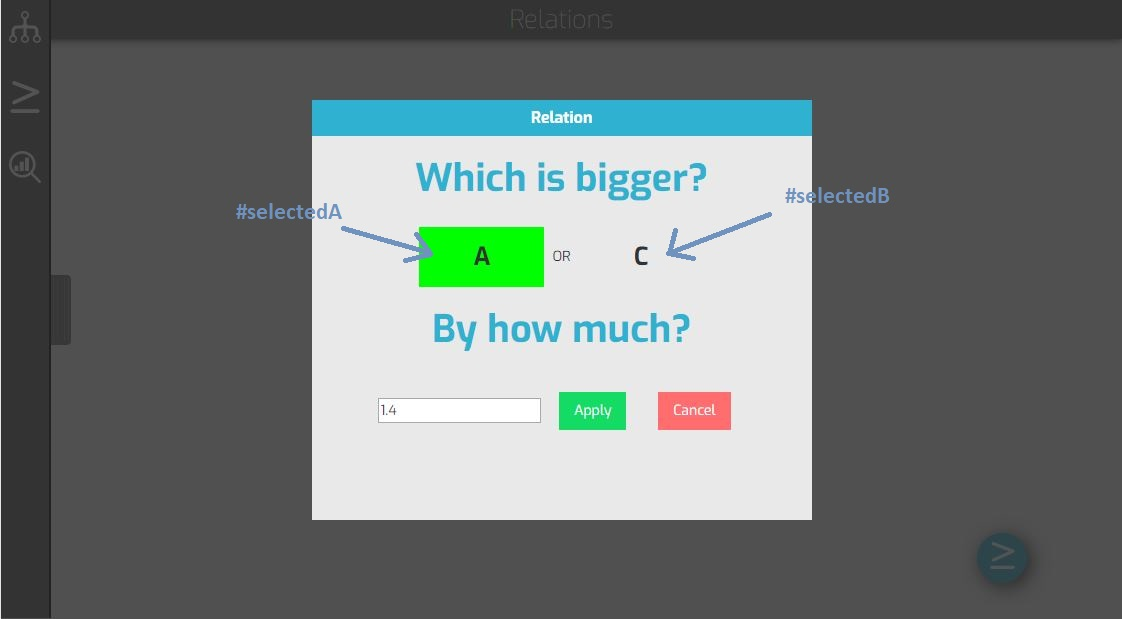
\includegraphics[width=\textwidth]{relationSelectionMechanism}
  \label{screenshot:relation selection}
\end{figure}

\noindent
\begin{minipage}[c]{\linewidth}
\begin{lstlisting}[basicstyle=\scriptsize, tabsize=4, frame=single, caption=Node Selection Variables, label=code:node selection variables]
var nodeA = null;
var nodeB = null;

var selectedA = $('#selectedA');
var selectedB = $('#selectedB');
\end{lstlisting}
\end{minipage}

\noindent
Then we need to know the order of selection (first selection or second selection). To determine the order of selection, If statement is used. See Code \ref{code:selection if statements}.

\noindent
\begin{minipage}[c]{\linewidth}
\begin{lstlisting}[basicstyle=\scriptsize, tabsize=4, frame=single, caption=Detect the order of selection, label=code:selection if statements]
		if(nodeA == null && nodeB == null){
			\\ this is the first selection
		}else if(nodeA != null && nodeB == null){
			\\ this is the second selection
		}else if(nodeA != null && nodeB != null){
			\\ the user already selected two nodes (a selection reset is required)
		}

\end{lstlisting}
\end{minipage}

\noindent
Referring  to Code \ref{code:selection if statements}:
\begin{itemize}
\item In the first selection, we simply find the selected node by id and store it in the variable \textbf{nodeA}, then change the selected node's background color for visual indication.
\item In the second selection, we find the selected node and store it in \textbf{nodeB}, then change the background color for the second node. After that, we change the text in \textbf{selectedA} and \textbf{selectedB} accordingly, then show the relation wizard.
\item In case two nodes are already selected, we need to reset the selections. To do so, we simply clear the selection variables, and re-draw the tree.
\end{itemize}
\noindent
The selecting function for this screen is stored in a variable called '\textbf{relationSelectionFunction}' then it is assigned to the callback attribute in chart configuration. To read about accessing the chart configuration, refer to section \ref{tree configuration}.
The complete code for Relation Screen selection function is shown in Code \ref{code:relationSelectionFunction}.

\noindent
\begin{minipage}[c]{\linewidth}
\begin{lstlisting}[basicstyle=\scriptsize, tabsize=4, frame=single, caption=Relation selection function, label=code:relationSelectionFunction]
var relationSelectionFunction = function(){
	$('.nodeClick').click(function(){
		if(nodeA == null && nodeB == null){
			findNode($(this).attr('id'), root);
			nodeA = targetNode;
			$(this).css({'background-color': '#2fb1d1', 'color': 'white'});
		}else if(nodeA != null && nodeB == null){
			$(this).css({'background-color': '#2fb1d1', 'color': 'white'});
			findNode($(this).attr('id'), root);
			nodeB = targetNode;
			
			selectedA.text(nodeA.text.name);
			selectedB.text(nodeB.text.name);
			
			relationWizard.show(250);
		}else if(nodeA != null && nodeB != null){
			nodeA = null;
			nodeB = null;			
			drawTree("#relateTreeChart", Tree);
		}
	});	
}

\end{lstlisting}
\end{minipage}
Note: '\textbf{relateTreeChart}' is the id for the html div element where the tree will be drawn.\\[12pt]

After the user selects two nodes, the relation wizard is shown, and the user is prompt to chose which node is bigger (in terms of weights). The user is also prompt to indicate 'by how much is one node bigger than the other'. For example, lets assume the user have two properties; property A and property C, and lets assume that property A is bigger than property C by forty percent (for example, if property C is 100 percent, then property A is 140 percent the size of property C). In this case we say that property A is 1.4 the size of property C. See Figure \ref{screenshot:relation selection}.\\
Once this relation is applied. It will be shown in the \textbf{Relation Tab}, and the user will have the ability to edit the relation or delete it, See Figure \ref{screenshot:relation tab}. For organization, all relations that are made under the same parents are grouped together.
\subsection{Analyzing}
In this screen, we want to highlight only the nodes that can be analyzed (nodes with more than two children), and the user should be able to click on the highlighted nodes only. Two features are implemented here, highlighting and selecting:

\begin{itemize}

\item The function to highlight nodes with more than two children is shown in Code \ref{code:highlightMatrixNodes}.

\noindent
\begin{minipage}[c]{\linewidth}
\begin{lstlisting}[basicstyle=\scriptsize, tabsize=4, frame=single, caption=Highlighting Matrix Nodes (nodes with more than 2 children), label=code:highlightMatrixNodes]
function highlightMatrixNodes(currentNode){
	if (countChildren(currentNode) > 2) {
		var node = $('#'+currentNode.HTMLid);
		node.css({'background-color': '#9EE7D9'});
    }
	currentNode.children.forEach(function (currentChild) {            
		highlightMatrixNodes(currentChild);
	});
    
}

\end{lstlisting}
\end{minipage}

\noindent
The function '\textbf{countChildren}' counts the number of children in a specific node. The code for the function \textbf{countChildren} is shown in Code \ref{code:countChildren}.

\noindent
\begin{minipage}[c]{\linewidth}
\begin{lstlisting}[basicstyle=\scriptsize, tabsize=4, frame=single, caption=countChildren function, label=code:countChildren]
function countChildren(node){
	counter = 0;
	node.children.forEach(function(child){
		counter++;
	});
	return counter;
}
\end{lstlisting}
\end{minipage}


\noindent
The function \textbf{highlightMatrixNodes} is recursive. It iterates through each node, and highlight it if it has more than two children. The highlighting technique in Code \ref{code:highlightMatrixNodes} works by first obtaining the html id of a node, then changing the background-color property of that node.


\item The selecting mechanism is stored in a variable called '\textbf{analyzeSelectionFunction}'. The complete code for the selecting mechanism for this screen is shown in Code \ref{code:analyzeSelectionFunction}.

\noindent
\begin{minipage}[c]{\linewidth}
\begin{lstlisting}[basicstyle=\scriptsize, tabsize=4, frame=single, caption=analyzeSelectionFunction function, label=code:analyzeSelectionFunction]
var analyzeSelectionFunction = function(){
	$('.nodeClick').click(function(){
		findNode($(this).attr('id'), root);
		numberOfChildren = countChildren(targetNode);
		if(numberOfChildren > 2){
			matrixTitle.text("Matrix (" + targetNode.text.name+")");
			printMatrix(targetNode.matrix, '#matrixView');
			matrixStatistics.text('');
			removeHighlights(targetNode.matrix)
			matrixWizard.show();
			
			// a list of inconsistencies is created (inconsList)
			calcInconsistancy(targetNode.matrix); 
		}
	});	
}
\end{lstlisting}
\end{minipage}
\noindent
As can be seen in Code \ref{code:analyzeSelectionFunction}, only nodes with more than two children are clickable. The \textbf{printMatrix} function will be explained later.
\end{itemize}

\subsection{Matrix Operations}
Many matrix operations are implemented, like printing and editing a matrix, deleting an element from a matrix, summing a matrix, and calculating elements weights from a matrix.

\noindent
We know that any matrix is a 2D array. Take for example the 5-by-5 matrix shown in Code \ref{code:matrixExample}. 


\noindent
\begin{minipage}[c]{\linewidth}
\begin{lstlisting}[basicstyle=\scriptsize, tabsize=4, frame=single, caption=Matrix Example, label=code:matrixExample]

Matrix = [
			 [A,B,C,D,E],
			 [F,G,H,I,J],
			 [K,L,M,N,O],
			 [P,Q,R,S,T],
			 [V,W,X,Y,Z]
		]

\end{lstlisting}
\end{minipage}
\\[6pt]

\noindent
In this system, every node has a matrix. Every time a child is added to a parent, that child is also added to the parent's matrix. See Code \ref{code:matrixConstruction}.

\noindent
\begin{minipage}[c]{\linewidth}
\begin{lstlisting}[basicstyle=\scriptsize, tabsize=4, frame=single, caption=Matrix construction, label=code:matrixConstruction]
for(i = 0 ; i < target.children.length ; i++){
		target.matrix[i] = [];
		for(j = 0 ; j < target.children.length ; j++){
			target.matrix[i][j] = 1;
		}
}
\end{lstlisting}
\end{minipage}

\noindent
The code in Code \ref{code:matrixConstruction} runs every time a node is added under a parent. It is a nested loop that is used to create a matrix of ones with a length that is equal to the number of children. So, if a node has four children, it would have a 4-by-4 matrix. See example in Code \ref{code:matrixExample2}.

\begin{minipage}[c]{\linewidth}
\begin{lstlisting}[basicstyle=\scriptsize, tabsize=4, frame=single, caption=Matrix Example 2, label=code:matrixExample2]
map[`node_root`].matrix = [
	[1,1,1,1],
	[1,1,1,1],
	[1,1,1,1],
	[1,1,1,1]
]
\end{lstlisting}
\end{minipage}

\subsubsection{Printing a matrix}

To represent a matrix as a table, we first need to know the length of its dimensions. For instance, a 4-by-4 matrix would have a length of four. If we look at a matrix as a table, its length would be the number of rows or columns, because every matrix has the same number of rows and columns. Then we can use a simple nested loop to draw the rows and columns of the matrix. Rows are arrays, and columns are elements. The outer loop should go through each row, and the inner loop should go through each column (element in an array).
A simple nested loop to draw a matrix can look like the code shown in Code \ref{code:matrixNestedLoop}.

\noindent
\begin{minipage}[c]{\linewidth}
\begin{lstlisting}[basicstyle=\scriptsize, tabsize=4, frame=single, caption=Matrix  nested loop, label=code:matrixNestedLoop]
for(i = 0; i < matrix.length; i++){
	for(j = 0; j < matrix.length; j++){
		//draw matrix[i][j]
	}
	//new line
}

\end{lstlisting}
\end{minipage}

\noindent
For this project however, we need more than just a simple draw. We need to draw elements names. We also need to draw the matrix as an html table. Plus we need to be able to access the values in the matrix as input fields. This adds a bit of complexity, but the concept of nested loop still holds. Take a look at the complexity of printing a matrix in this system in the flowchart in Figure \ref{diagram:printMatrix}. Also see the JS function \textbf{printMatrix} shown in Code \ref{code:printMatrix}.

\begin{figure}[H]
  \caption{Matrix Printing Flowchart}
  \centering
  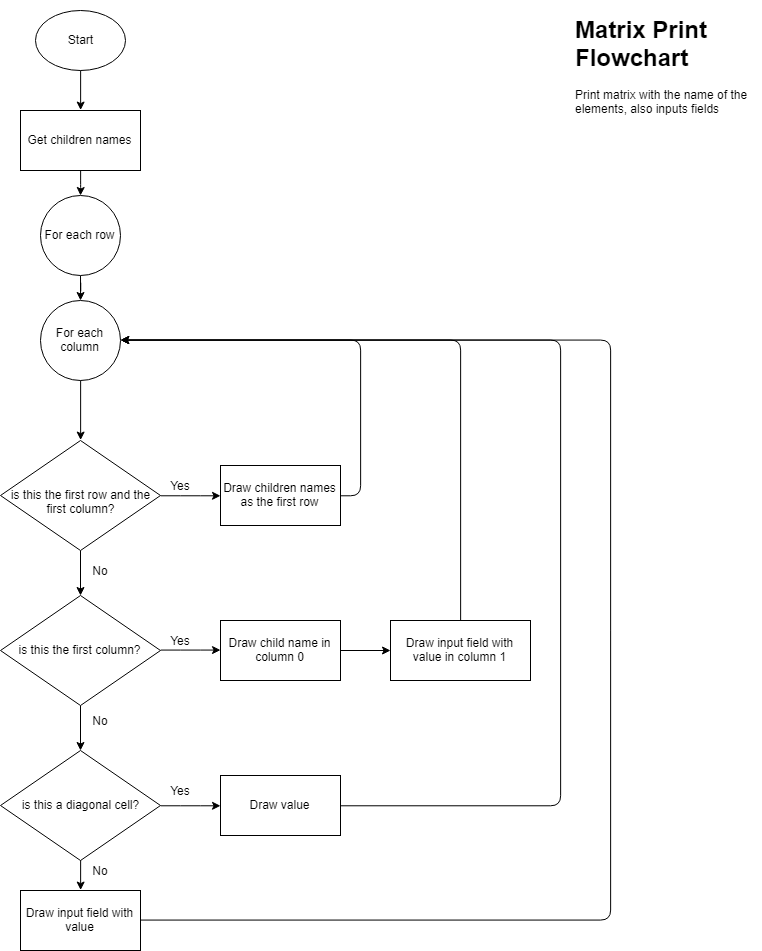
\includegraphics[width=\textwidth]{printMatrix}
  \label{diagram:printMatrix}
\end{figure}

\noindent
\begin{minipage}[c]{\linewidth}
\begin{lstlisting}[basicstyle=\scriptsize, tabsize=4, frame=single, caption=printMatrix Function, label=code:printMatrix]
function printMatrix(node, targetDiv){
	var matrix = node.matrix;
	var children = node.children;
	var elementsNames = [];
	
	var table = "";
	
	//get elements names in an array
	children.forEach(function(child){
		elementsNames.push(child.text.name);
	});
	
	for(i = 0 ; i < matrix.length; i++){
		for(j = 0 ; j < matrix.length; j++){
			if(i == 0 && j == 0){
				table += "<tr><td class='elementName'>~</td>";
				elementsNames.forEach(function(element){
					table += "<td class='elementName'>"+element+"</td>";
				});
				table += "</tr><tr>";
			}
			if(j == 0){
				table += "<td class='elementName'>"+elementsNames[i]+"</td>";
			}
			if(i != j){
				//input id = cell_ij_input
				table += "<td id='cell_"+i+j+"' data-i='"+i+"' data-j='"+j+"'
 onClick='cellClick(this.id)' ><input id='cell_"+i+j+"_input' class='cellInput' type='text' value='"+matrix[i][j]+"' readonly></td>";
			}else{
				table += "<td>"+matrix[i][j]+"</td>";
			}	
		}
		table += "</tr>";
	}
	targetDiv = $(targetDiv);
	targetDiv.text('');
	targetDiv.append(table);
}

\end{lstlisting}
\end{minipage}

\noindent
\textbf{printMatrix} function takes two arguments:
\begin{itemize}
\item \textbf{node}: is the node that we want to print its matrix.
\item \textbf{targetDiv}: is the html div id of where we want the matrix to be drawn.
\end{itemize}

\noindent
An output example of the function \textbf{printMatrix} would look similar to the matrix shown in Figure \ref{matrixExample}.

\begin{figure}[H]
  \caption{Matrix print example}
  \centering
  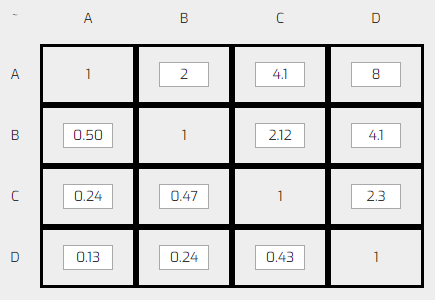
\includegraphics[width=0.5\textwidth]{matrixExample}
  \label{matrixExample}
\end{figure}
\noindent
Notice the input fields and the corresponding names for elements at the top of the table and the left side.
\noindent

When the user click on a node, the inconsistency for that node will be calculated and stored, along with all the traids for the matrix associated with it. This is broken into the following steps:

First, we know that every relation produces a traid with three values (X, Y, and Z). We also know that each traid can be calculated using the formula described by Koczkodaj in \cite{DBLP} and shown in Figure \ref{formula:inconsistencyValue}. Therefore a JSON structure to save each consistency is implemented as shown in Code \ref{code:inconsistency structure}.

\begin{figure}[H]
  \caption{Inconsistency Value Formula}
  \centering
  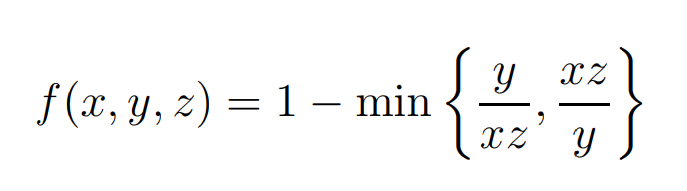
\includegraphics[width=0.5\textwidth]{inconsistancyFormula}
  \label{formula:inconsistencyValue}
\end{figure}

\noindent
\begin{minipage}[c]{\linewidth}
\begin{lstlisting}[basicstyle=\scriptsize, tabsize=4, frame=single, caption=inconsistency JSON structure, label=code:inconsistency structure]
{
	incons: (1-Math.min((x*z)/y,y/(x*z))).toFixed(5),
	x:[i,j],
	y:[i,k],
	z:[j,k]
}
\end{lstlisting}
\end{minipage}






\section{Testing}

\section{Publishing}

\newpage
\printbibliography

\end{document}




